\documentclass[11pt,a4paper,titlepage,oneside]{article}
\usepackage{LabProtocol}

\exercise{Exercise III}

% enter your data here
\groupno{14}
\authors{
  Anna Balla, Matr. Nr. 11709469 \par
  {\small e11709469@student.tuwien.ac.at} \par
  Philipp Geisler, Matr. Nr. 11775812 \par
  {\small e11775812@student.tuwien.ac.at}
}


\begin{document}

\maketitle

%%%%%%%%%%%%%%%%%%%%%%%%%%%%%%%%%%%%%%%%%%%%%%%%%%%%%%%%%%%%%%%%%%%%%%%%%%%%%%%%
%%%%%%%%%%%%%%%%%%%%%%%%%%%%%%%%%%%%%%%%%%%%%%%%%%%%%%%%%%%%%%%%%%%%%%%%%%%%%%%%

\begin{figure}[ht!]
  \centering
  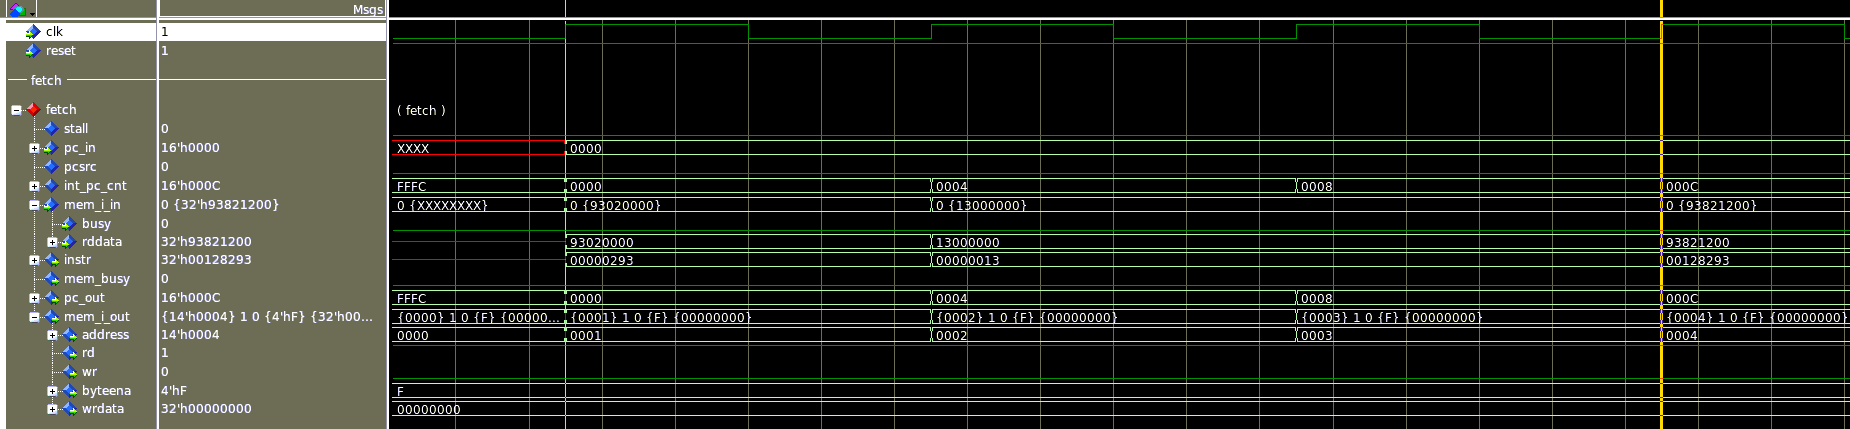
\includegraphics[width=1.0\linewidth]{fig/fetch_0_015_to_0_045.png}
  \caption{Simulation screenshot for Listing~\ref{lst:asmnofwd}. 0.015 us to 0.045 us. }
  \label{fig:sim}
\end{figure}

Make sure the following signals are visible in Figure~\ref{fig:sim} and the 
signal values are readable:
the program counter in the fetch stage, the instruction being fetched, the 
content of register \texttt{x5} and the fields \texttt{address}, \texttt{rd}, 
\texttt{wr}, \texttt{byteena}, and \texttt{wrdata} in the \texttt{mem\_out} 
signal coming out of the pipeline in the memory stage.

\begin{figure}[ht!]
	\centering
	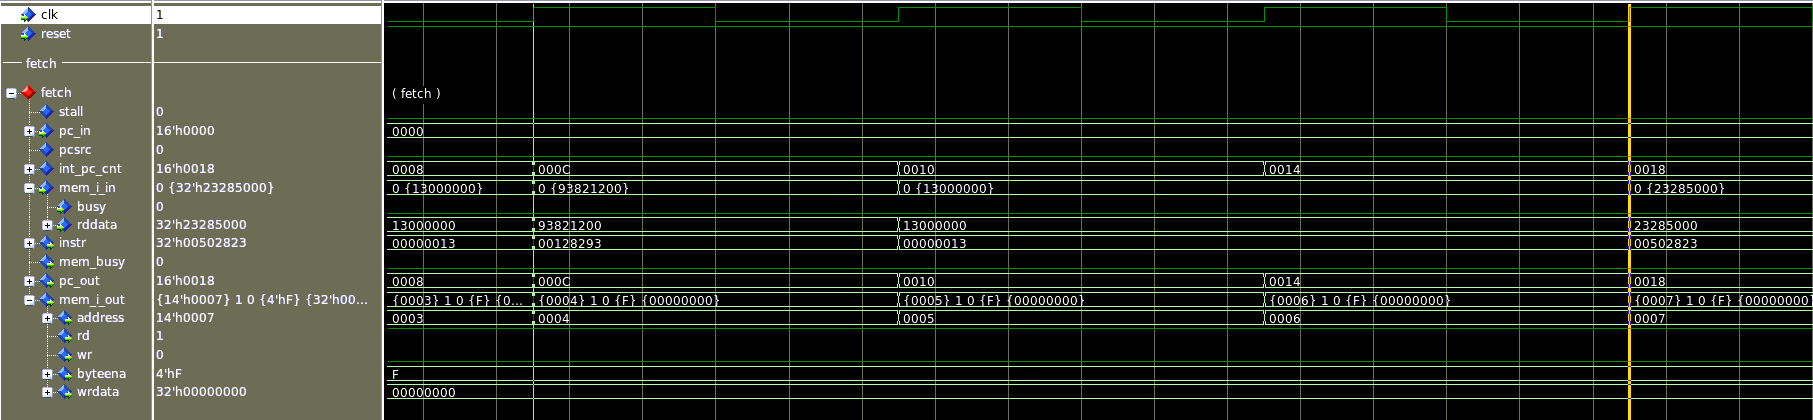
\includegraphics[width=1.0\linewidth]{fig/fetch_0_045_to_0_075.png}
	\caption{Simulation screenshot from 0.045 us after start-up until 0.075 us.}
	\label{fig:sim_2}
\end{figure}

\begin{figure}[ht!]
	\centering
	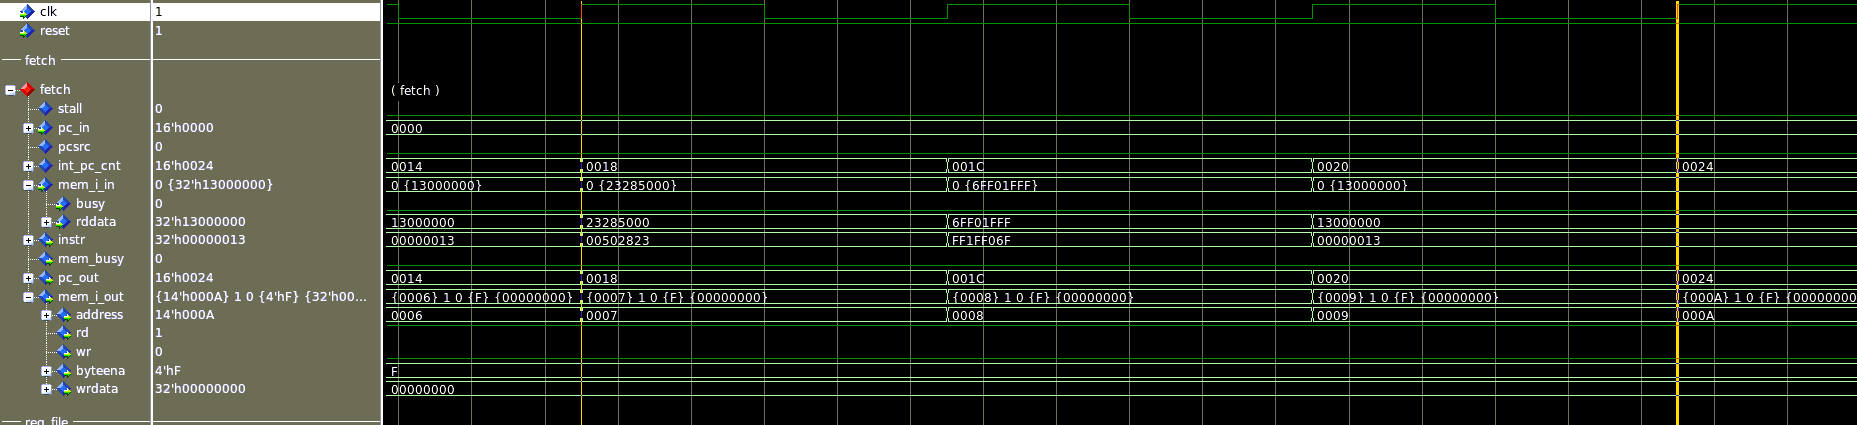
\includegraphics[width=1.0\linewidth]{fig/fetch_0_075_to_0_105.png}
	\caption{Simulation screenshot from 0.075 us after start-up until 0.105 us.}
	\label{fig:sim_3}
\end{figure}

\begin{figure}[ht!]
	\centering
	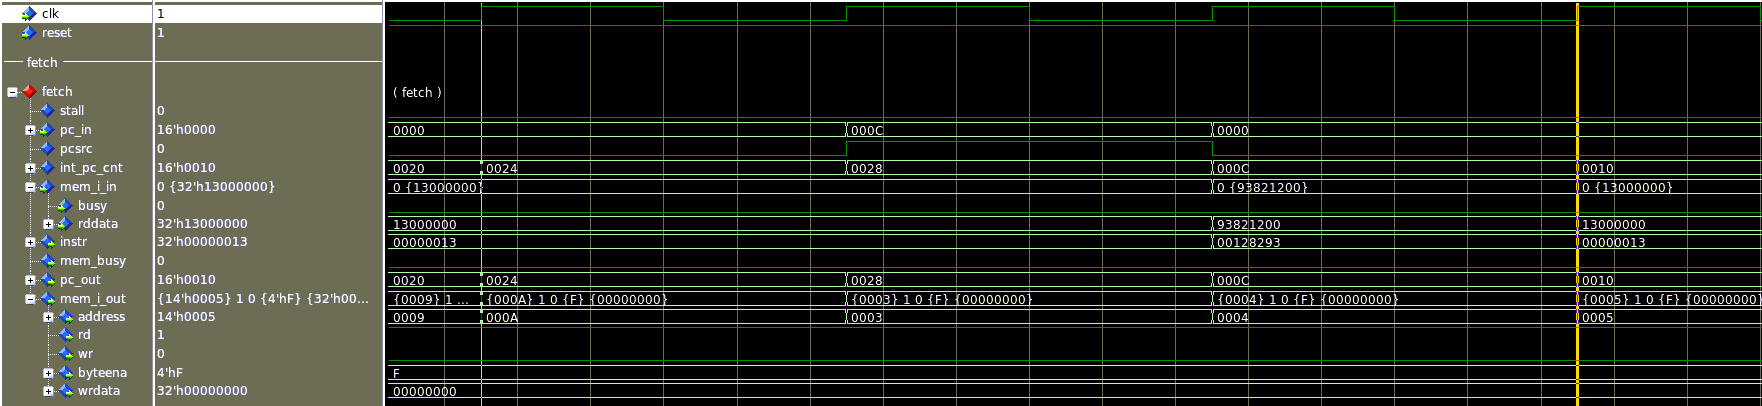
\includegraphics[width=1.0\linewidth]{fig/fetch_0_105_to_0_135.png}
	\caption{Simulation screenshot from 0.105 us after start-up until 0.135 us.}
	\label{fig:sim_4}
\end{figure}

The figures ~\ref{fig:sim}, ~\ref{fig:sim_2}, ~\ref{fig:sim_3} and  ~\ref{fig:sim_4} show one iteration
of the whole code presented in \textit{submission.S} and the behavior the code triggers in the fetch stage. \par 
 
\begin{figure}[ht!]
	\centering
	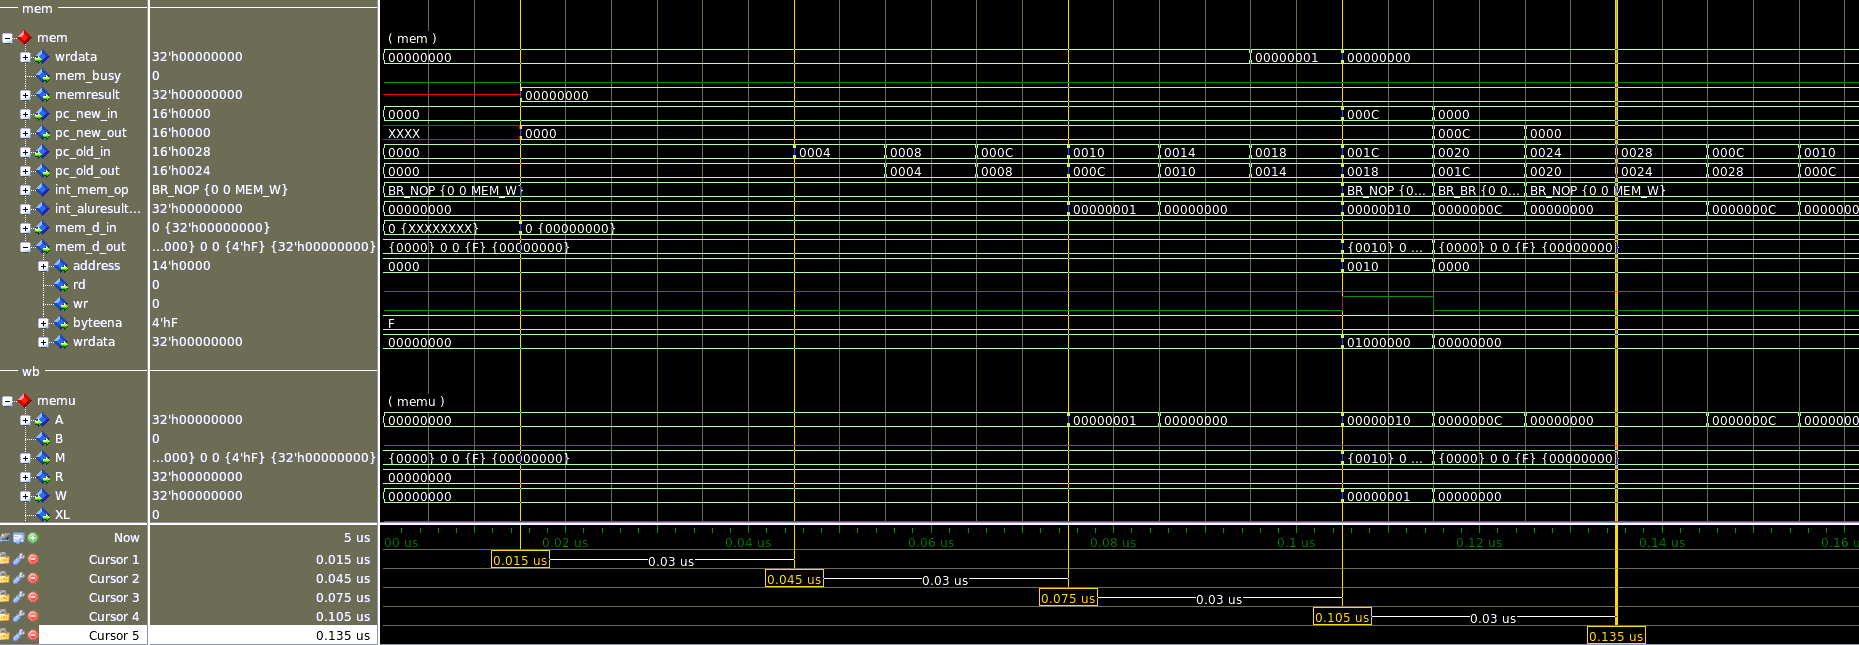
\includegraphics[width=1.0\linewidth]{fig/mem_full_transition.png}
	\caption{Simulation screenshot showing the behavior of the mem stage during one iteration.}
	\label{fig:mem_full}
\end{figure}


\begin{figure}[ht!]
	\centering
	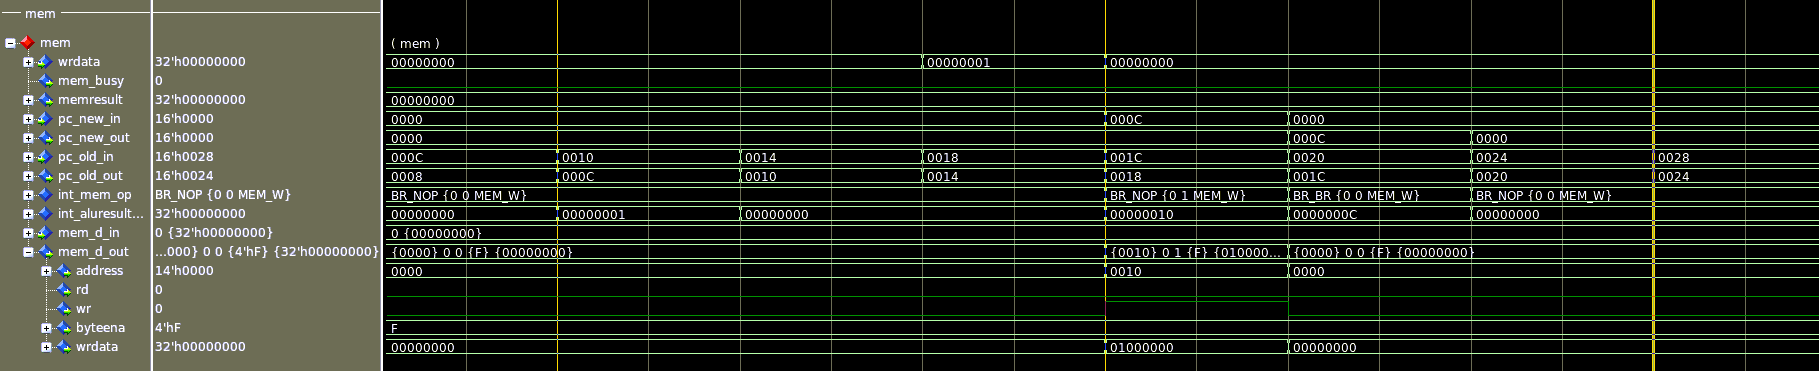
\includegraphics[width=1.0\linewidth]{fig/mem_0_075_to_0_135.png}
	\caption{Simulation screenshot from 0.075 us to 0.135 us of the mem stage.}
	\label{fig:mem_act}
\end{figure}

The figures ~\ref{fig:mem_full} and ~\ref{fig:mem_act} show whats going on in the mem stage. 


\begin{figure}[ht!]
	\centering
	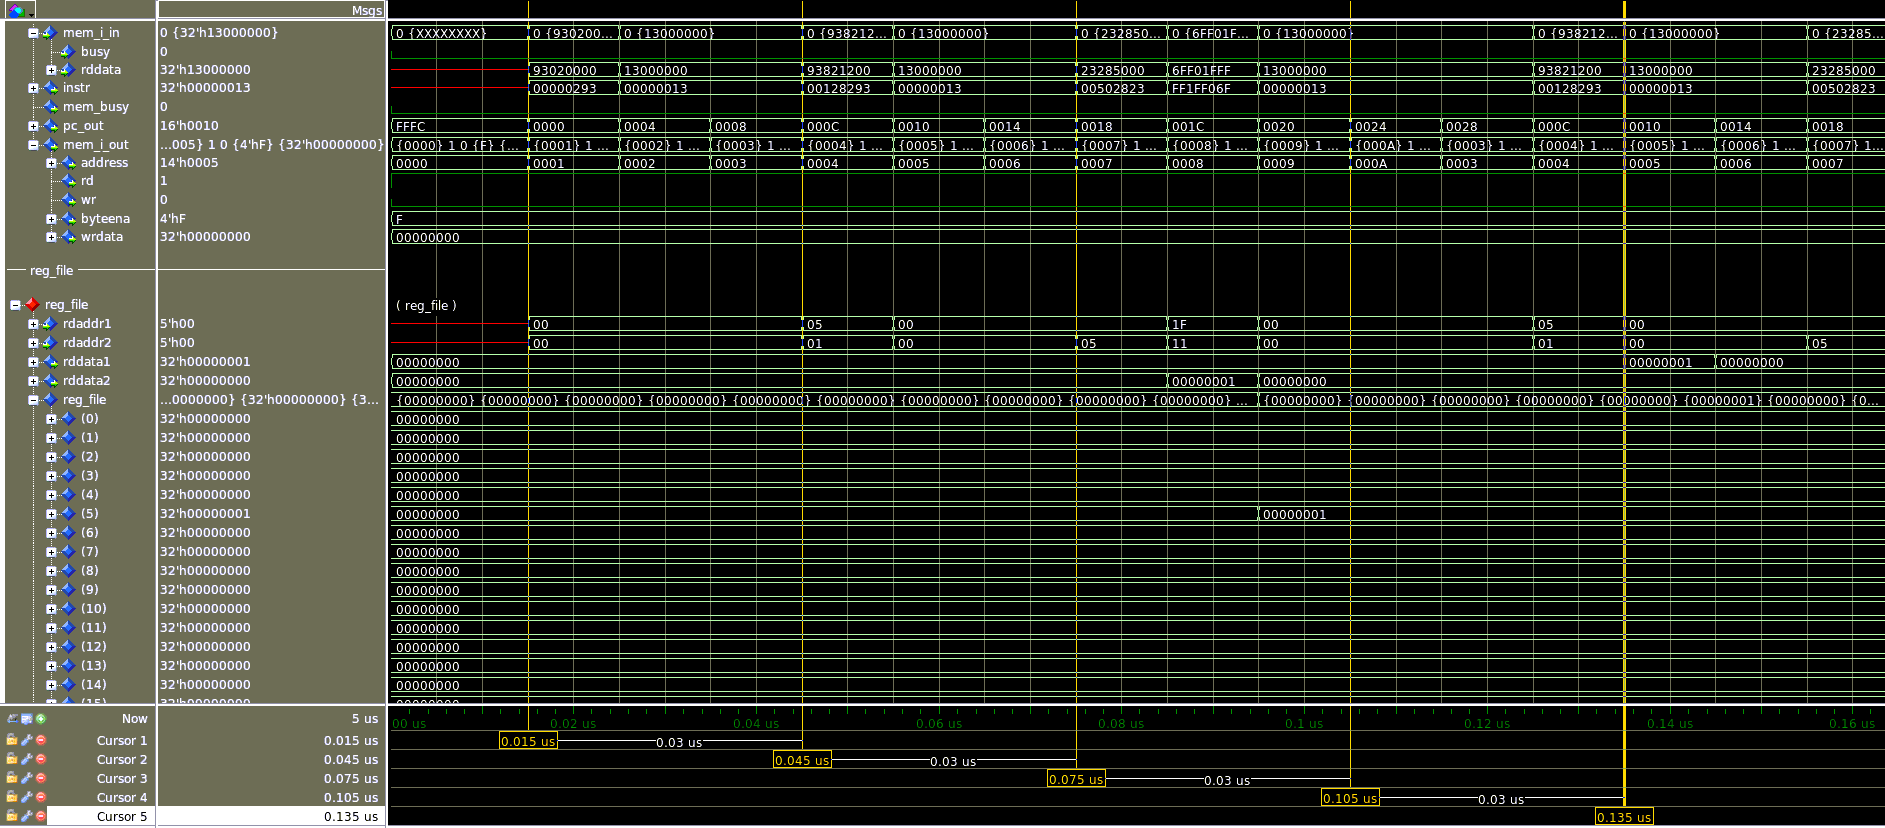
\includegraphics[width=1.0\linewidth]{fig/regfile_0_to_0_135.png}
	\caption{Simulation screenshot from 0 us after start-up until 0.135 us.}
	\label{fig:regf}
\end{figure}

Figure ~\ref{fig:regf} shows what's going on in the regfile during the iteration. One can clearly see
that the output of the addi instruction is written back to the regfile. If you simulate longer than the 
first iteration one can see that the assembly-code essential implements a counter that is being
incremented. 


\begin{lstlisting}[language=,mathescape=false,float=ht,caption={Assembler example without forwarding},label=lst:asmnofwd]
        addi x5, x0, 0
        nop
        nop
loop:
        addi x5, x5, 1
        nop
        nop
        sw x5, 16(x0)
        jal x0, loop
        nop
        nop
        nop
\end{lstlisting}
%%%%%%%%%%%%%%%%%%%%%%%%%%%%%%%%%%%%%%%%%%%%%%%%%%%%%%%%%%%%%%%%%%%%%%%%%%%%%%%%
%%%%%%%%%%%%%%%%%%%%%%%%%%%%%%%%%%%%%%%%%%%%%%%%%%%%%%%%%%%%%%%%%%%%%%%%%%%%%%%%

\end{document}
